\newline
\title{LEZIONE 19 15/04/2020}\newline
\textbf{link} \href{https://web.microsoftstream.com/video/8edecaf9-c042-4da8-905e-0412c9f62daa?list=user&userId=faa91214-a6f5-40d7-8875-253fd49b8ce1}{clicca qui}
\subsection{Studio di una funzione complessa razionale fratta $G(s)$ di variabile complessa su una curva chiusa}
Data una generica curva $\Gamma$ su cui si muove la variabile $s$, applicando l'operatore $G()$ otteniamo una nuova curva $\Delta$ su cui viaggia la variabile $G(s)$:\newline
[immagine dagli appunti del prof]
\begin{center}
    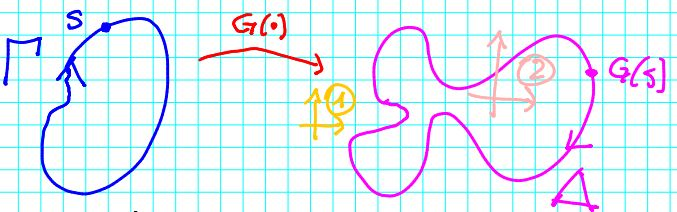
\includegraphics[height=3cm]{../lezione19/img1.JPG}
\end{center}
Domanda: $\Delta$ circonda l'origine del piano complesso dove si muove $G(s)$? Cioè siamo nella situazione $1$ (in giallo) o $2$ (in rosa)? \newline
\[
    G(s) = \frac{\dots (s-z) \dots}{\dots (s-p) \dots} \Rightarrow arg(G(s)) = \dots + arg(s-z) \dots - arg(s-p)
\]
Casi possibili:
\begin{itemize}
    \item \textbf{CASO 1:}\newline
    $\Gamma$ circonda un polo $p$ di $G(S)$ in senso orario (o)\newline
    [immagine dagli appunti del prof]
    \begin{center}
        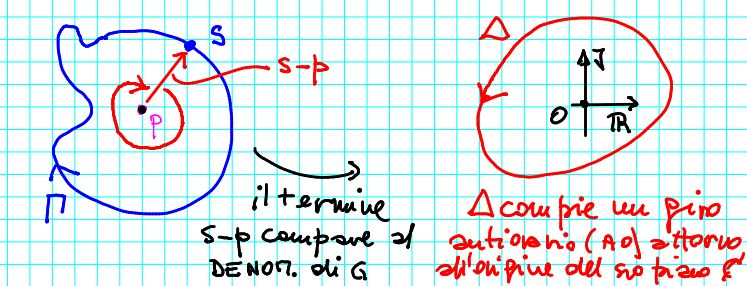
\includegraphics[height=3cm]{../lezione19/img2.JPG}
    \end{center}
    Il termone $s-p$ compare al denominatore di $G$. $\Delta$ compie un giro antiorario (ao) attorno all'origine del suo piano complesso.
    \item \textbf{CASO 2:}\newline
    $\Gamma$ circonda in senso orario uno zero $z$ di $G(s)$, allora $\Delta$ compie un giro orario attorno all'origine del suo piano complesso.
    \item \textbf{CASO 3:}\newline
    $\Gamma$ non circonda nè zeri nè poli di $G(s)$, allora $\Delta$ non circonda l'origine del suo piano complesso.\newline
    [immagine dagli appunti del prof]
    \begin{center}
        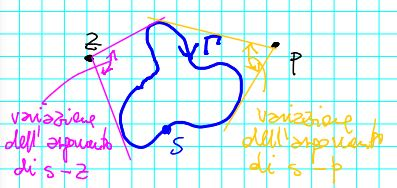
\includegraphics[height=3cm]{../lezione19/img3.JPG}
    \end{center}
\end{itemize}
Da questi casi deduciamo che il numero di giri antiorari che l'immagine $\Delta$ della curva $\Gamma$ attraverso $G(s)$ compie attorno all'origine del suo piano complesso è uguale al numero di poli di $G$ circondati da $\Gamma$ in senso orario meno il numero di zeri di $G$ circondati da $\Gamma$ in senso orario.\newline
\newline
\textbf{oss.} ($1$ giro orario) = -($1$ giro antiorario) e viceversa.